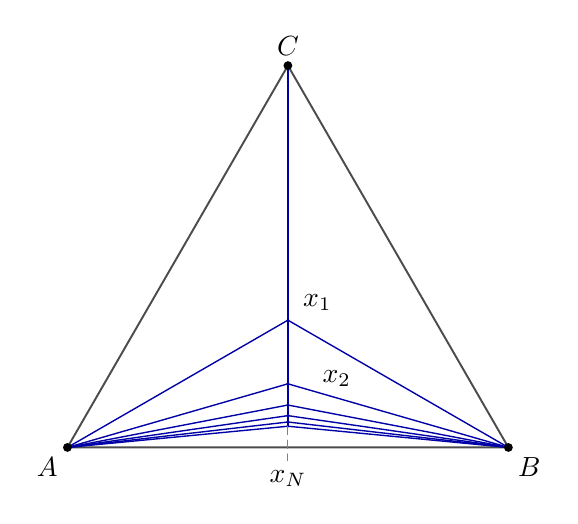
\begin{tikzpicture}[x=5.6cm,y=5.6cm,line cap=round,line join=round]
 \coordinate (A) at (0,0);
 \coordinate (B) at (1,0);
 \coordinate (C) at (0.5,0.8660254038);
 \draw[black!70,line width=0.7pt] (A)--(B)--(C)--cycle;
 \foreach \j in {1,...,6}{
   \coordinate (X\j) at (0.5,{0.2886751346/\j});
   \draw[blue!65!black,line width=0.5pt] (A)--(X\j)--(B);
 }
 \draw[blue!65!black,line width=0.5pt] (C)--(X1);
 \foreach \j in {2,...,6}{
   \pgfmathtruncatemacro{\prev}{\j-1}
   \draw[blue!65!black,line width=0.5pt] (X\prev)--(X\j);
 }
 \foreach \p in {A,B,C}{\fill[black] (\p) circle[radius=0.010];}
 \foreach \j in {1,...,6}{\fill[blue!65!black] (X\j) circle[radius=0.0035];}
 \node[below left] at (A) {$A$};
 \node[below right] at (B) {$B$};
 \node[above] at (C) {$C$};
 \node[above right,xshift=2pt] at (X1) {$x_1$};
 \node[right,xshift=9pt,yshift=2pt] at (X2) {$x_2$};
 \draw[black!50,densely dashed,thin] (X6)--(0.5,-0.03);
 \node[below] at (0.5,-0.03) {$x_N$};
\end{tikzpicture}
